\chapter{Grundlagen}
\thispagestyle{standard}
\pagestyle{standard}
\renewcommand{\footrulewidth}{0.4pt}
\lfoot{\small Refik Kerimi}

Wie in Kapitel \ref{chap:Einleitung} beschrieben, hat der stetige Zuwachs von \acl{SP}s \acs{SP}s \cite{Geraetenutzung} zum Umdenken bei der Planung und beim Entwickeln von Webapplikationen geführt.
Zu beginn jedes Projektes steht die Entscheidung an, welche Technologien und Tools zur Entwicklung verwendet werden sollen um die bestmögliche Ergebnis zu erhalten.
Wenn die falschen Methoden gewählt werden, kann das zu gravierenden Fehlern in der Applikation führen, die sich erst mit Fortdauer der produktiven Verwendung ersichtlich machen.
Entscheidet man sich für eine Anwendung die auf das Betriebssystem zugeschnitten ist oder doch für eine plattformübergreifende Webanwendung. Beide haben Vorteile und Nachteile und diese werden im Zuge dieser Arbeit betrachtet. Der Kern der Arbeit stellt, aber die von Google entwickelten \acs{PWA} \cite{PWA} da. Die \acs{PWA}s sollen den Spagat zwischen diesen beiden Anwendungen schaffen. Eventuell könnte diese neue Form der Appentwicklung die traditionelle Technologien gar zur Gänze ablösen?
Der Trend in den letzten Jahren geht in Richtung der Mobilen Nutzung und da ist das \acl{SP} klar wie, in Abbildung \ref{fig:Internetnutzung} und \ref{fig:Smartphonenutzung} dargestellt, voran.  

\begin{figure}[h]
	\centering
	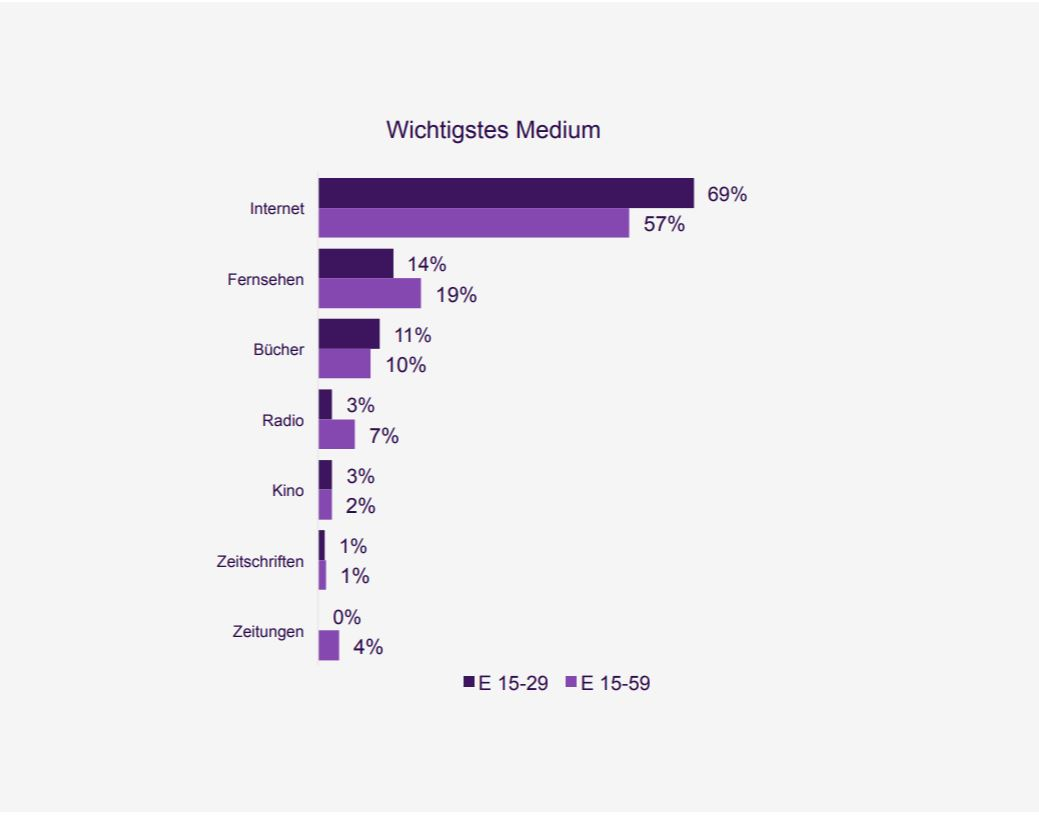
\includegraphics[width=14cm]{BilderAllgemein/Internetnutzung}\medskip
	\caption{Internetnutzung \cite{Geraetenutzung}}
	\label{fig:Internetnutzung}
\end{figure}

\begin{figure}[h]
	\centering
	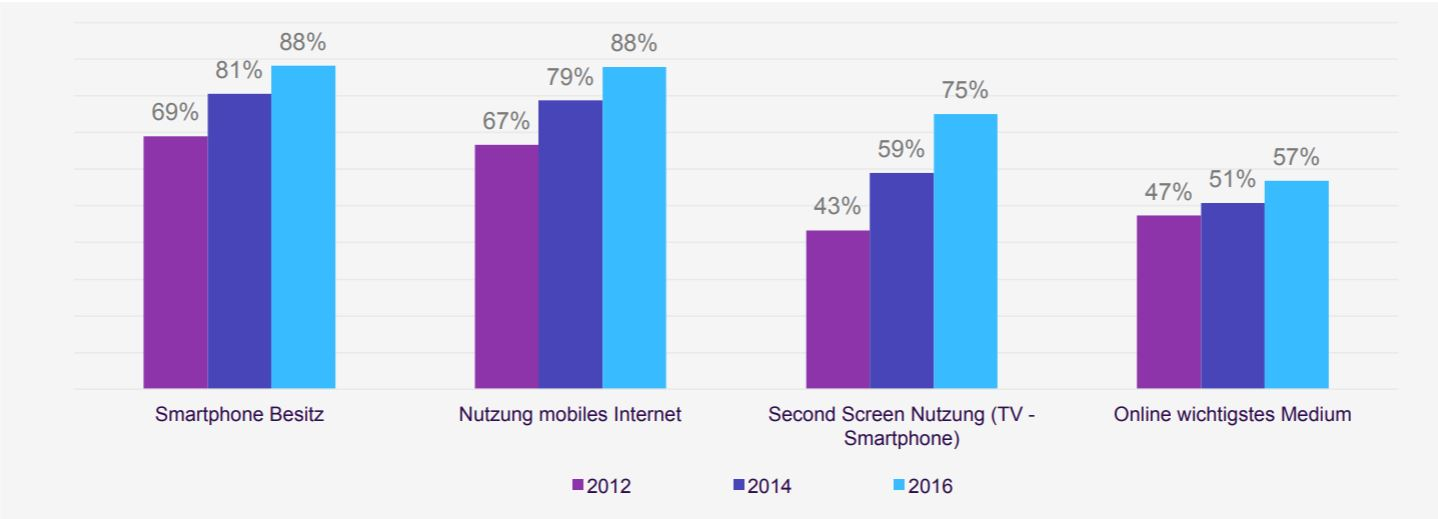
\includegraphics[width=14cm]{BilderAllgemein/SmartPhoneNutzung}\medskip
	\caption{Smartphonenutzung \cite{Geraetenutzung}}
	\label{fig:Smartphonenutzung}
\end{figure}







\section{Geschichte Softwareentwicklung}
Um die Geschichte der Softwareentwicklung darstellen zu können müssen wir als aller ersten die Frage stellen "Was ist Software?" und was wie ist eine Software definiert.
Diese Frage stellen sich sicherlich alle mal die zum ersten Mal in ihrem Leben mit dieser Technologie in Berührung kommen. Eine genau Definition zu finden ist schwierig da die Software für die Gesamtheit eines Produktes steht . In \cite{WasistSoftware} ist die Softwaretechnik wie folgt definiert:
\begin{quote}
\glqq Zielorientierte Bereitstellung und systematische Verwendung von Prinzipien, Methoden und Werkzeugen für
die arbeitsteilige, ingenieurmäßige Entwicklung und Anwendung
von umfangreichen Softwaresystemen. Zielorientiert bedeutet die
Berücksichtigung z.B. von Kosten, Zeit, Qualität.\grqq (\cite{WasistSoftware} Seite 17).
\end{quote}
Im laufe der Jahre wurden verschiedenste Software entwickelt die mehr oder weniger nützlich für unseren Alltag waren.
Der Begriff Software wurde 1958 vom US-amerikanischen Statistiker John W. Turkey eingeführt.
Zu Beginn bildeten Software und Hardware eine Einheit. Erst nach der Entscheidung durch die US Regierung, dass IBM die Hardware und die Software separat verrechnen werden sollte.
Die Software bildet das Gehirn eines eines Computers. 
Nach der Entscheidung der US-Regierung entstanden erstmals rein Softwareorienttiere Unternehmen wie Microsoft oder SAP \cite{Microsoft} \cite{SAP}. 


\newpage

\section{Mobile Applikationen}
Anfang des neues Jahrtausends war die Vorstellung, dass das Mobiltelefon für uns sehr viele alltäglichen Aufgaben erledigt unvorstellbar, doch heute können wir uns das Leben ohne 
Mobiltelefon kaum vorstellen.
Wir organisieren unser Leben damit und steuern unsere Haushaltsgerät, unser Garagentor und verbinden uns mit unserem Auto usw. all diese Möglichkeiten werden durch Apps ermöglicht.
Die Apps werden im allgemeinen in 3 Kategorien aufgeteilt
Native-, Web- und Hybridapps. 

\subsection{Native Apps}\label{chap:Native Apps}
\acl{NA}s (NA) (deutsch; angepasste Anwendung) ist speziell für eine Plattform angepasste Anwendung. 
Diese werden speziell für ein bestimmtes Betriebssystem konzipiert und haben in der Regel zugriff auf alle Ressourcen eines Gerätes \cite{NativeApp}.
Hauptsächlich werden zur Programmierung für Mobile Geräte die Hochsprachen Java (Android) und Swift(IOS) verwendet. Native Apps können in App Stores heruntergeladen  werden, die bekanntesten sind Apple Store und Google Play \cite{Hochsprachen}.

\subsection{Webapplikationen}\label{chap:Webapplikationen}
Im Gegensatz zu den \acs{NA}s sind \acl{WA} (\acs{WA}) speziell Programmierte Webseiten \cite{Hochsprachen}.
\acs{WA} funktionieren nach dem Server-Client Prinzip und werden vom Browser aufgerufen. In der Regel werden \acs{WA}s auf der Basis von \acs{JS}, \acs{CSS} und \acs{HTML5} entwickelt. Die Verarbeitung erfolgt auf dem Webserver oder auf der Cloud. 
Client seitig werden die Ergebnisse der Datenverarbeitung angezeigt. Der größte Vorteil ist sicherlich der unkomplizierte Zugang im Gegensatz zu den \acs{NA}s \cite{WebApps}.
Durch die Einführung von Responsive Frameworks wie z.B.: Bootstrap, SemantikUI oder Foundation um nur die bekanntesten zu nennen, wurde die Webentwicklung vielseitiger in der Verwendung. Durch diese Technologien können viele Gerätegrößen mit wenig Aufwand abgedeckt werden \cite{CSS}. 

\subsection{Hybridapplikationen}
\acl{HyApp}s (\acs{HyApp}) verbinden die Eigenschaften den in Kapitel \ref{chap:Native Apps} und \ref{chap:Webapplikationen} genannten Technologien. Zum einen verwenden Sie die Webbasierende Client-Server Technologie zum anderen kann man mit einer \acs{HyApp} auf Gerätefunktioonen wie Kamera und Kalender zugreifen \cite{HybridApps}. 

\subsection{Progressive Web Apps}
\acl{PWA} sind im Grunde eine Weiterentwicklung von einer \acs{WA}. Diese Technologie der Webentwicklung wird durch die immer schneller Wachsende Welt der Webapplikationen immer wichtiger. 
Dem User wird das Gefühl gegeben er arbeitet mit einer \acs{NA}. Das Herausragende dabei ist es,im Gegensatz zu einer \acs{HyApp}, dass jede bestehende \acs{WA} in eine \acs{PWA} umgebaut werden kann.
Durch hinzufügen eines Manifest Files und eines \acl{SW} (\acs{SW}) werden Features hinzugefügt, die es ermöglichen Offline zu arbeiten oder das Icon der App auf den Desktop oder Home-Bildschirm zu speichern \cite{PWA}.
Google definiert die \acs{PWA} wie folgt:


\begin{itemize}
    \item  \textbf{Progressive} - Funktioniert für alle User unabhängig vom Browser
	\item  \textbf{Responsive} - Passt sich jedem Gerät an	
	\item  \textbf{Verbindungsunabhängig} - funktioniert auch bei schlechtem oder gar keinem Internetzugang
	\item  \textbf{App-like} - fühlt sich an wie eine \acs{NA}
	\item  \textbf{Akteull} - Durch die Wartung des \acs{SW} immer auf dem aktuellsten Stand
	\item  \textbf{Sicher} - wird nur über HTTPS bereitgestellt
	\item  \textbf{Erkennbar} - erkennbar dank das W3C Manifest durch Suchmaschinen
	\item  \textbf{Wiedereinschaltbar} - wird durch die Funktion Push Notfication
	\item  \textbf{Installierbar} - Ermöglicht das hinzufügen auf dem Startbildschirm
	\item  \textbf{Verteilbar } - Einfache Freigabe über URL \cite{PWAAdjectives}
\end{itemize}. 




\newpage

